\paragraph{Sơ đồ tuần tự luồng bắt buộc xác thực 2FA khi đăng nhập}

Luồng nghiệp vụ này mô tả
chi tiết quá trình bắt buộc xác thực mã TOTP
sau khi
đăng nhập.

\begin{figure}[H]
\centering
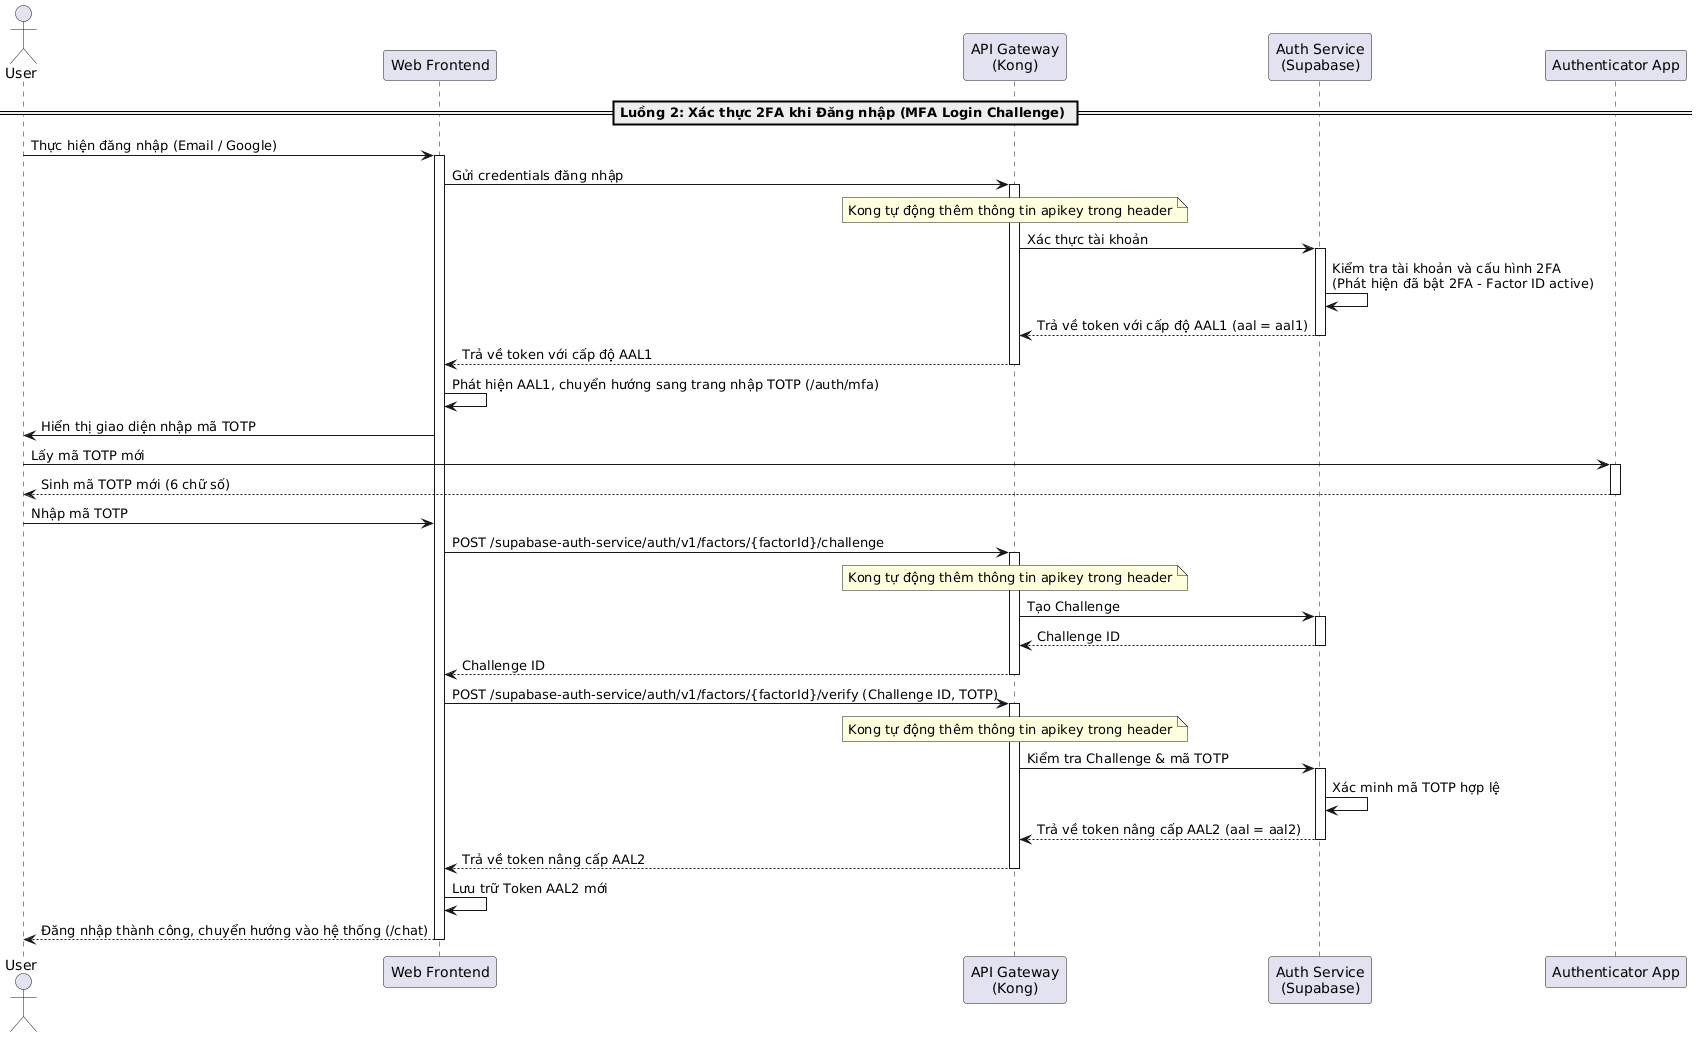
\includegraphics[width=0.95\textwidth]{contents/Sequence/UML-Sequence-UserMfaLoginChallenge.png}
\caption{Sơ đồ tuần tự luồng bắt buộc xác thực 2FA khi đăng nhập}
\end{figure}

\begin{table}[H]
\centering
\renewcommand{\arraystretch}{1.3}

\begin{tabular}{|l|l|p{5cm}|}
\hline
\textbf{Thành phần} & \textbf{Phân loại} & \textbf{Vai trò trong hệ thống} \\ \hline
User & Actor & Người dùng thực hiện đăng nhập. \\ \hline
Web Frontend & Component & Giao diện web Next.js. \\ \hline
API Gateway (Kong) & Component & Cổng API chuyển tiếp các yêu cầu API. \\ \hline
Auth Service (Supabase) & Microservice & Dịch vụ Supabase kiểm tra và sinh challenge, nâng cấp token AAL1 lên AAL2. \\ \hline
Authenticator App & External App & Ứng dụng sinh mã TOTP. \\ \hline
\end{tabular}
\caption{Các thành phần tham gia luồng bắt buộc xác thực 2FA khi đăng nhập}
\end{table}

\subparagraph{Mô tả tổng quan}

\begin{itemize}

\item \textbf{Đăng nhập bước đầu:}
Khi người dùng đăng nhập,
hệ thống chỉ cấp mã phiên đăng nhập ở mức độ bảo mật cơ bản.

\item \textbf{Yêu cầu xác thực lớp thứ hai:}
Giao diện phát hiện mức độ bảo mật của phiên đăng nhập chưa đạt yêu cầu
bảo mật cấp 2,
lập tức chặn quyền truy cập
và chuyển hướng người dùng sang trang yêu cầu nhập mã xác thực hai lớp.

\item \textbf{Nhập mã xác thực:}
Người dùng điền mã xác thực lấy từ ứng dụng trên điện thoại di động.
Giao diện gửi yêu cầu xác minh qua cổng API tới Auth Service.

\item \textbf{Nâng cấp phiên đăng nhập:}
Sau khi xác minh thành công,
Auth Service nâng cấp phiên đăng nhập lên mức độ bảo mật cấp 2,
cấp mã đăng nhập mới gửi
về giao diện để người dùng
có thể truy cập đầy đủ
các chức năng trò chuyện chính của hệ thống.
\end{itemize}
